\subsection{تخمین پارامتر کانال یاو}
برای اصلاح پارامترها یاو چندین آزمایش انجام شد و با استفاده از خروجی‌هایآزمایش و جعبه‌ابزاز
\lr{Parameter Estimator}
پارامترها اصلاح شدند.
برای آزمایش یاو همه‌ی موتورها با دور یکسان شروع به حرکت کردند و خروجی‌هایسنسور داده برداری شد. سپس، مدل و پارامترهای داده برداری شده به جعبه‌ابزار
\lr{Parameter Estimator}
داده شد. نتایج آزمایش‌های کانال یاو بعد از اصلاح پارامترها در شکل
%(\ref{yaw_ps1})
آورده شده است.

\begin{figure}[H]
	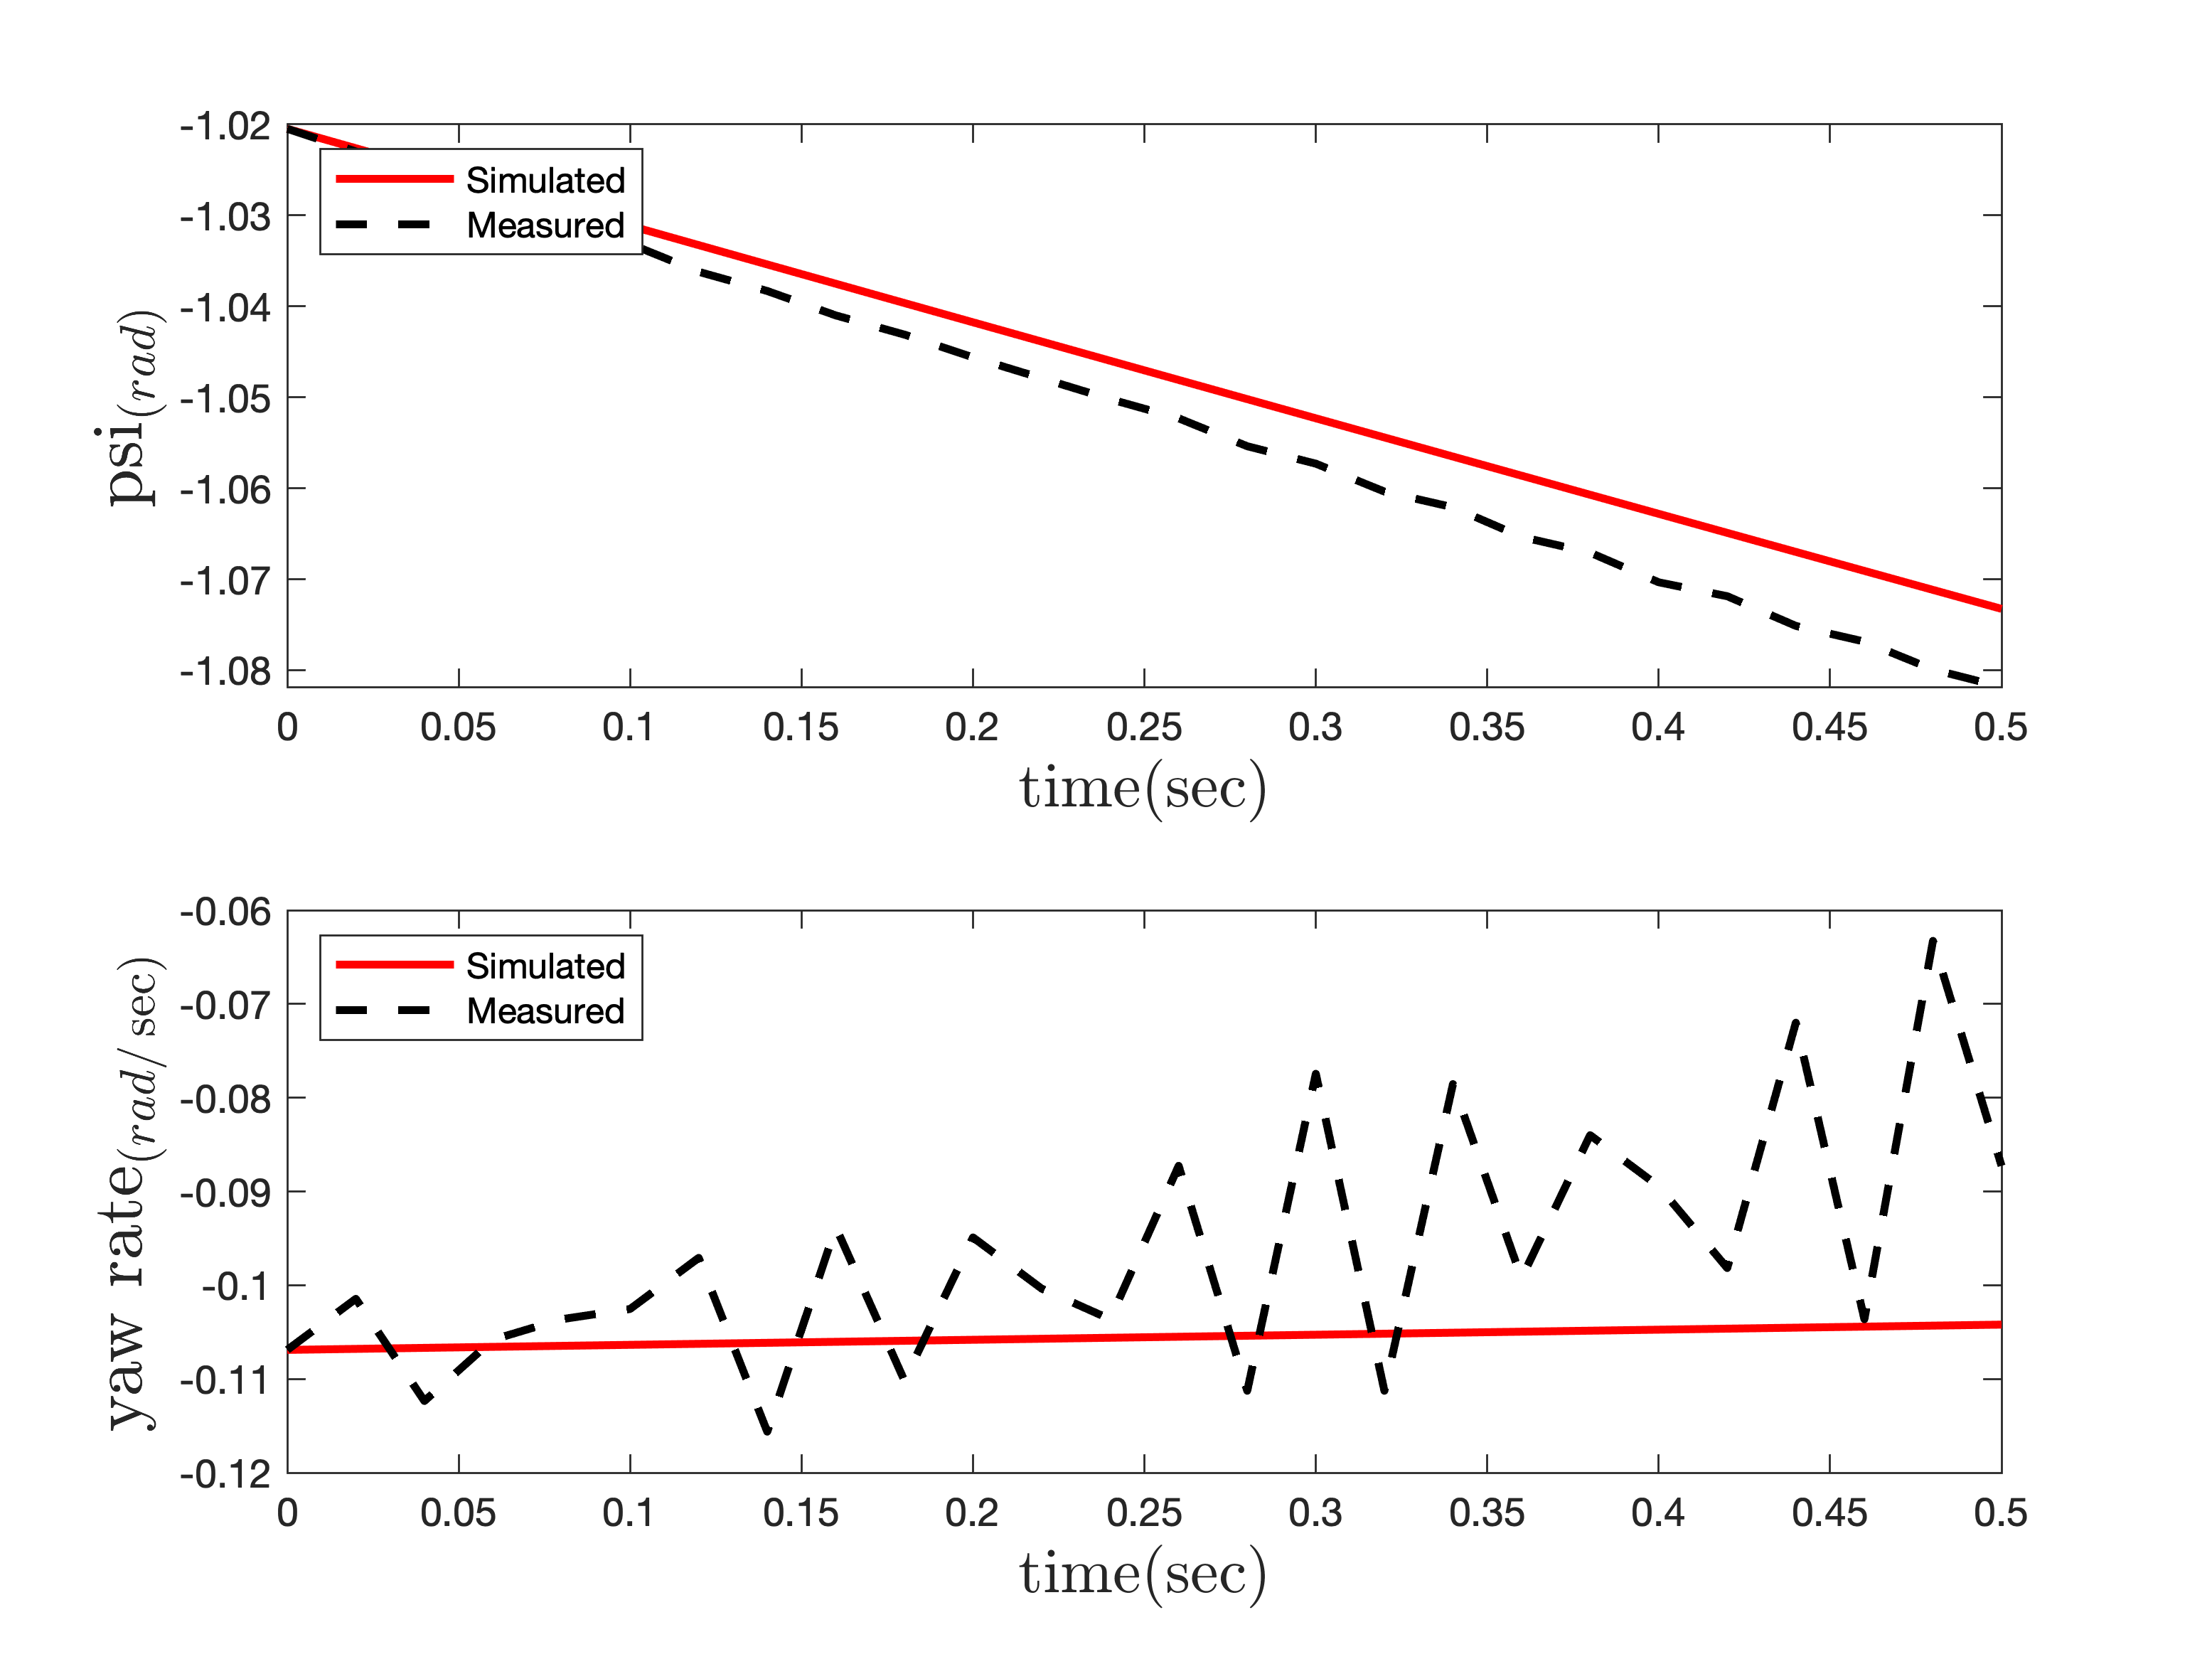
\includegraphics[width=12cm]{../../Figures/RCP/yaw_parameter_estimation/RCP_yaw_S1.png}
	\centering
	\caption{مقايسه خروجی‌های آزمايش اول و خروجی‌های شبیه‌سازی پس از تخمین پارامترهای کانال یاو}
	\label{yaw_ps1}
\end{figure}